% Created 2014-03-12 Wed 13:10
\documentclass[a4paper,8pt]{article}
\usepackage[utf8]{inputenc}
\usepackage[T1]{fontenc}
\usepackage{fixltx2e}
\usepackage{graphicx}
\usepackage{longtable}
\usepackage{float}
\usepackage{wrapfig}
\usepackage{rotating}
\usepackage[normalem]{ulem}
\usepackage{amsmath}
\usepackage{textcomp}
\usepackage{marvosym}
\usepackage{wasysym}
\usepackage{amssymb}
\usepackage{hyperref}
\tolerance=1000
\usepackage[margin=1.0in]{geometry}
\author{N-CRITSER}
\date{\textit{<2014-03-12 Wed>}}
\title{HW5-EVAL.ORG}
\hypersetup{
  pdfkeywords={},
  pdfsubject={},
  pdfcreator={Emacs 23.4.1 (Org mode 8.2.4)}}
\begin{document}

\maketitle
\tableofcontents



\section{SEARCH COMPARISON}
\label{sec-1}
For the two problems compared (missionaries-and-cannibals still under construction)
Breadth-first-search solved both within a comparable amount of time but expanded
far more nodes than the two constrained variants of Depth-first-search.  General
Depth-first-search (DFS)  performed so poorly that I was unable to solve the problems
due to system time outs.  According to system monitor statistics,   
DFS timed out after 12 min and using 95\% of system ram on the farmer problem and 
after 10 min 95\% ram on \textbf{water-jug}.  
Unlike its  variants, which solved the problem within milliseconds, 
while barely consuming any ram. 
Breadth-first-search (BFS) solved the problems in milliseconds, but expanded many more 
nodes than the Depth-first-search-duplicate-node-detection (DFSDND) and Depth-first-search-
depth-limit (DFSDL).  For the farmer problem BFS expanded 239 nodes , as opposed to 
DFSDND and DFSDL which both only expanded 8 nodes for the same problem.  

     Pruning the search trees using either a hueristic value for depth limiting or by 
systematically preventing expansion of duplicate nodes effectively decreases the number
of searchable paths.  This type of algorithmic improvement can diminish shortcomings in a 
basic algorithm, as can be seen with DFS as compared to DFSDND \& DFSDL.  By limiting the 
deficiencies of DFS, we expand far fewer nodes than BFS , to arrive at a solution path. Its
logical to assume that this kind of improvement can make an asymptotically important difference
as search spaces grow.  



\subsection{CHART}
\label{sec-1-1}
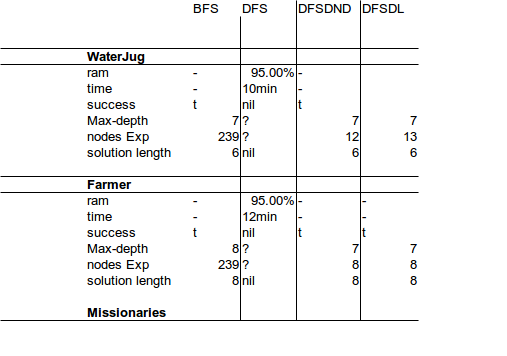
\includegraphics[angle=0,width=8cm]{./image2993.png}



\subsection{OUTPUT FROM TESTS}
\label{sec-1-2}

\subsubsection{BREADTH-FIRST-SEARCH}
\label{sec-1-2-1}
\begin{enumerate}
\item WATER-JUG
\label{sec-1-2-1-1}
\begin{verbatim}
Performing breadth first search on problem water jug.
#<SEARCH-STATISTICS #x302001084ABD>
Class: #<STANDARD-CLASS SEARCH-STATISTICS>
Wrapper: #<CCL::CLASS-WRAPPER SEARCH-STATISTICS #x302000FDE98D>
Instance slots
NODES-VISITED: 239
MAXIMUM-LENGTH-OF-NODE-LIST: 114
LENGTH-OF-SOLUTION: 6
MAXIMUM-DEPTH: 7
%#<NODE #x302001136EED>
Class: #<STANDARD-CLASS NODE>
Wrapper: #<CCL::CLASS-WRAPPER NODE #x302000FED9FD>
Instance slots
STATE: #<JUG-STATE #x302001136F9D>
PROBLEM: #<PROBLEM #x30200105BA7D>
PATH: (DUMP-2 FILL-2-FROM-5 DUMP-2 FILL-2-FROM-5 DUMP-2 EMPTY-5-INTO-2)
ANCESTORS: NIL
#<NODE #x302001136EED>
\end{verbatim}

\item FARMER
\label{sec-1-2-1-2}
\begin{verbatim}
Performing breadth first search on problem the farmer, the fox, the goose, and the grain.
#<SEARCH-STATISTICS #x30200104E40D>
Class: #<STANDARD-CLASS SEARCH-STATISTICS>
Wrapper: #<CCL::CLASS-WRAPPER SEARCH-STATISTICS #x302000FDE98D>
Instance slots
NODES-VISITED: 239
MAXIMUM-LENGTH-OF-NODE-LIST: 127
LENGTH-OF-SOLUTION: 7
MAXIMUM-DEPTH: 8
%#<NODE #x302001059E2D>
Class: #<STANDARD-CLASS NODE>
Wrapper: #<CCL::CLASS-WRAPPER NODE #x302000FED9FD>
Instance slots
STATE: #<FARMER-STATE #x302001059EED>
PROBLEM: #<PROBLEM #x302000F772ED>
PATH: (FARMER-TAKES-GOOSE
        FARMER-TAKES-SELF
        FARMER-TAKES-FOX
        FARMER-TAKES-GOOSE
        FARMER-TAKES-GRAIN
        FARMER-TAKES-SELF
        FARMER-TAKES-GOOSE)
ANCESTORS: NIL
#<NODE #x302001059E2D>
\end{verbatim}
\end{enumerate}

\subsubsection{DEPTH-FIRST-SEARCH-DUPE-DETECT}
\label{sec-1-2-2}

\begin{enumerate}
\item WATER-JUG
\label{sec-1-2-2-1}
\begin{verbatim}
Performing depth first search with duplicate node detection on problem water jug.
#<SEARCH-STATISTICS #x30200120C9AD>
Class: #<STANDARD-CLASS SEARCH-STATISTICS>
Wrapper: #<CCL::CLASS-WRAPPER SEARCH-STATISTICS #x302000FDE98D>
Instance slots
NODES-VISITED: 12
MAXIMUM-LENGTH-OF-NODE-LIST: 2
LENGTH-OF-SOLUTION: 6
MAXIMUM-DEPTH: 7
%#<NODE #x30200120AE5D>
Class: #<STANDARD-CLASS NODE>
Wrapper: #<CCL::CLASS-WRAPPER NODE #x302000FED9FD>
Instance slots
STATE: #<JUG-STATE #x30200120AF0D>
PROBLEM: #<PROBLEM #x30200105BA7D>
PATH: (DUMP-2 FILL-2-FROM-5 DUMP-2 FILL-2-FROM-5 DUMP-2 EMPTY-5-INTO-2)
ANCESTORS: NIL
\end{verbatim}
\item FARMER
\label{sec-1-2-2-2}
\begin{verbatim}
Performing depth first search with duplicate node detection on problem the farmer, the fox, the goose, and the grain.
#<SEARCH-STATISTICS #x3020010EC18D>
Class: #<STANDARD-CLASS SEARCH-STATISTICS>
Wrapper: #<CCL::CLASS-WRAPPER SEARCH-STATISTICS #x302000F5964D>
Instance slots
NODES-VISITED: 8
MAXIMUM-LENGTH-OF-NODE-LIST: 2
LENGTH-OF-SOLUTION: 7
MAXIMUM-DEPTH: 7
%#<NODE #x3020010EA79D>
Class: #<STANDARD-CLASS NODE>
Wrapper: #<CCL::CLASS-WRAPPER NODE #x302000F632DD>
Instance slots
STATE: #<FARMER-STATE #x3020010EA85D>
PROBLEM: #<PROBLEM #x302000F772ED>
PATH: (FARMER-TAKES-GOOSE
        FARMER-TAKES-SELF
        FARMER-TAKES-FOX
        FARMER-TAKES-GOOSE
        FARMER-TAKES-GRAIN
        FARMER-TAKES-SELF
        FARMER-TAKES-GOOSE)
ANCESTORS: NIL
\end{verbatim}
\end{enumerate}
\subsubsection{DEPTH-FIRST-WITH-DEPTH-LIMIT}
\label{sec-1-2-3}

\begin{enumerate}
\item WATER-JUG
\label{sec-1-2-3-1}
\begin{verbatim}
Performing depth first search with depth limit on problem water jug.
#<SEARCH-STATISTICS #x30200128D0BD>
Class: #<STANDARD-CLASS SEARCH-STATISTICS>
Wrapper: #<CCL::CLASS-WRAPPER SEARCH-STATISTICS #x302000FDE98D>
Instance slots
NODES-VISITED: 13
MAXIMUM-LENGTH-OF-NODE-LIST: 4
LENGTH-OF-SOLUTION: 6
MAXIMUM-DEPTH: 7
%#<NODE #x30200128B20D>
Class: #<STANDARD-CLASS NODE>
Wrapper: #<CCL::CLASS-WRAPPER NODE #x302000FED9FD>
Instance slots
STATE: #<JUG-STATE #x30200128B2BD>
PROBLEM: #<PROBLEM #x30200105BA7D>
PATH: (DUMP-2 FILL-2-FROM-5 DUMP-2 FILL-2-FROM-5 DUMP-2 EMPTY-5-INTO-2)
ANCESTORS: NIL
\end{verbatim}

\item FARMER
\label{sec-1-2-3-2}
\begin{verbatim}
Performing depth first search with depth limit on problem the farmer, the fox, the goose, and the grain.
#<SEARCH-STATISTICS #x3020011E196D>
Class: #<STANDARD-CLASS SEARCH-STATISTICS>
Wrapper: #<CCL::CLASS-WRAPPER SEARCH-STATISTICS #x302000FDE98D>
Instance slots
NODES-VISITED: 8
MAXIMUM-LENGTH-OF-NODE-LIST: 4
LENGTH-OF-SOLUTION: 7
MAXIMUM-DEPTH: 7
%#<NODE #x30200121F89D>
Class: #<STANDARD-CLASS NODE>
Wrapper: #<CCL::CLASS-WRAPPER NODE #x302000FED9FD>
Instance slots
STATE: #<FARMER-STATE #x30200121F95D>
PROBLEM: #<PROBLEM #x302000F772ED>
PATH: (FARMER-TAKES-GOOSE
        FARMER-TAKES-SELF
        FARMER-TAKES-FOX
        FARMER-TAKES-GOOSE
        FARMER-TAKES-GRAIN
        FARMER-TAKES-SELF
        FARMER-TAKES-GOOSE)
ANCESTORS: NIL
#<NODE #x30200121F89D>
\end{verbatim}
\end{enumerate}
\section{CRYPTARITHMETIC}
\label{sec-2}
\begin{verbatim}
  ABCDE
+ FBCDE
-------
 FGHEJB
\end{verbatim}
\begin{verbatim}
X: {A,B,C,D,E,F,G,H,J}
D: {0...9}
C: 
c1:   <E + E = B + x10>
c2:   <x10 + D + D = J + x100>
c3:   <x100 + C + C = E + x1000>
c4:   <x1000 + B + B = H + x10000>
c5:   <x10000 + A + F = G + x100000>
c6:   <{B,H} != odd> (all are results of 2*x = K )
c7:   <{F} = 1 > -- if (+ 99999 99999)= 199998 max carry is 1
\end{verbatim}

\begin{verbatim}
E{0,2,3,4,5,6,7,8,9}  ----> E=0 ------------>B=0 :( E=B=0 
E{2,3,4,5,6,7,8,9 }  -----> E=2 ----------->B{0,4,6,8} B=4----------> H{0,6,8} H=8
------------> C{0,2,3,4,5,6,7,8,9} C=6 --->6+6=12 -->E=2 ---> B=4 4=4=1=9 = H!=8 :(

E{2,3,4,5,6,7,8,9 }  ---->E=4 ---------->B{0,2,6,8} B=8 -----> H{0,2,6} H=6 (8+8=16)--
---> C{0,2,3,5,7,9} C=7 --->7+7=14  -->1+8+8= 17= H!= 16 :(

E{2,3,4,5,6,7,8,9 } E=6 ---> C{2,3,4,5,7,8,9} C=3 3+3=6----> B{2,4,8} B=2 CARRY1 --
-->H{0,4,8} H=4  ------> D{5,7,9} D=5 5+5=10 -->J=0---->C+C+1 = 7!= E =6 :(

B{2,6,8} ----->B=6  -------->E{3,8} E=3--------> D{2,4,5,7,8,9}D=7--->J=4 CARRY1---
--->C{2,3,4,5,7,8,9} 1+C+C=3 C!=1 :(
\end{verbatim}
% Emacs 23.4.1 (Org mode 8.2.4)
\end{document}
